\documentclass[journal]{new-aiaa}
%\documentclass[journal]{new-aiaa} for journal papers
\usepackage[utf8]{inputenc}
\usepackage{graphicx}
\usepackage{amsmath}
\usepackage[version=4]{mhchem}
\usepackage{siunitx}
\usepackage{longtable,tabularx}
\usepackage{float}
\setlength\LTleft{0pt} 
\graphicspath{{}}

% \usepackage{lineno}
% \linenumbers

% \title{Global Optimization - Depth-First Search}
\title{Global Steering for Control Moment Gyro Clusters\\ using Heuristic Variable Search Techniques}


\author{Charalampos Papakonstantinou\footnote{Ph.D Student, Department of Mechanical Engineering and Aeronautics, c\_papakonstantinou@upnet.gr}, Vaios J.Lappas\footnote{Research Professor, Department of Mechanical Engineering and Aeronautics, Senior Member AIAA, vlappas@upatras.gr}, Hanspeter Schaub\footnote{Professor, Aerospace Engineering Sciences Department, Colorado Center for Astrodynamics Research, University of Colorado, hanspeter.schaub@colorado.edu} and Vasilios Kostopoulos\footnote{Professor, Department of Mechanical Engineering and Aeronautics, Director of the Laboratory: Laboratory of Applied Mechanics and Vibrations, kostopoulos@upatras.gr}}
\affil{University of Patras, Rio, Greece, 26504}

\begin{document}

\maketitle

\begin{abstract}
This paper addresses the problem of singularity avoidance in a 4-control moment gyroscope (CMG) cluster as used for the attitude control of a satellite. A global search algorithm is developed that adjusts the null motion added upon the Singularity Robust Inverse (SRI) steering law. Its principal characteristic is that it uses global information gathered from the whole manoeuvre compared to most conventional techniques that consider only some local information, near the current gimbal configuration for the optimization.  The method is implemented using a ternary tree structure and a heuristic algorithm optimizes a cost function that depends on the manipulability index, the time spent in the vicinity of singularity, the quaternion error and the gimbal rates. Specific measures are taken to decrease the execution time of the algorithm even for long manoeuvres, without the need of a visit histogram. In addition, the tuning of only two variables can drastically change the execution time and the computational resources needed. The numerical simulation used to evaluate the algorithm indicates that the elliptic singularity can sufficiently be avoided and the algorithm drives the system fast away from the singularity with an overall performance improvement.
\end{abstract}
\section*{Nomenclature}

{\renewcommand\arraystretch{1.0}
\noindent\begin{longtable*}{@{}l @{\quad=\quad} l@{}}
$\textbf{H}$  & spacecraft angular momentum vector \\
$\dot{\textbf{H}}$ & time derivative of spacecraft angular momentum vector \\
$\textbf{h}$   & CMG angular momentum vector \\
$\dot{\textbf{h}}$ & time derivative of CMG angular momentum vector \\
$\textbf{h}_c$ & commanded momentum vector\\
$h_m$ & mean maximum angular momentum \\
$\boldsymbol{\omega}$& spacecraft angular velocity vector \\
$\textbf{T}_{ex}$ & external torques vector \\
$\textbf{T}_{cmg}$ & torque vector created by CMG \\
$\textbf{T}_c$ & control torque vector \\
$h_0$ & magnitude of momentum of each flywheel  \\
$\beta$   & skew angle \\
$\boldsymbol{\delta}$  & gimbal angles vector \\
$\dot{\boldsymbol{\delta}}$  & time derivative of gimbal angles vector  \\
$\dot{\boldsymbol{\delta}}_{sat}$ & saturated gimbal rates vector\\
$\dot{\boldsymbol{\delta}}_{Null}$ & time derivative of gimbal angles vector that belongs in the null space \\
$\dot{\delta}_{th}$ & gimbal rates saturation threshold\\
$\textbf{A}(\boldsymbol{\delta})$  & Jacobian matrix\\
$\textbf{A}^{\#}(\boldsymbol{\delta})$  & inverse of the Jacobian matrix\\
$\textbf{q}$ & quaternion vector\\
$\dot{\textbf{q}}$ & time derivative of quaternion vector\\
$\textbf{q}_{err}$ & quaternion error vector\\
$\textbf{q}_{des}$ & desired quaternion vector\\
$\textbf{q}^{*}_{des}$ & conjugate of quaternion vector\\
$\textbf{q}_{ini}$ & initial quaternion vector\\
$\textbf{q}_{i}$ & quaternion vector in $i^{th}$ iteration\\
$K_p, K_\omega$ & PD gains\\
$\lambda_0$ & steering law gain\\
$w$ & manipulability index\\
$w_{th}$ & manipulability index threshold\\
$CF$ & cost function \\
$g_1, g_2, g_3, g_4$ & cost function coefficients\\
$w_{mean}$ & mean value of manipulability along the trajectory\\
$T_{w<w_{th}}$ & term proportional to the time the
manipulability index is below a specific threshold\\
$||\textbf{q}_{err}^v||_{max}$ & maximum norm of the quaternion error vector across the trajectory\\
$T_{max\{\dot\delta_1, \dot\delta_2, \dot\delta_3, \dot\delta_4\}>\dot \delta_{th}}$ & term proportional to the time the gimbal rates exceed a specific threshold\\
$D$ & tree depth\\
$\textbf{L}$ &  null motion set\\
%!!!!!!!!!!!!!! INCLUDE k_i here !!!!!!!!!!!!!!!!%
$k_{max}$ & maximum null motion value\\
$skip_{rate}$ & number of children skipped by the algorithm\\
$skip_{th}$ & threshold of children skipped by the algorithm \\
$dt$ & time-step\\
$I_{exec}$ & execution index\\
\end{longtable*}}

\section{Introduction}
\lettrine{C}{ontrol} Moment Gyroscopes (CMGs) are widely used in spacecraft control for manoeuvring and they have been successfully employed for a wide range of space missions \cite{futuremissions,defendini,wie2008space}. A single gimbal control moment gyroscope is a device consisted of a spinning wheel that rotates at a constant rate attached on a gimbal motor. Taking advantage of the torque amplification effect, they are ideal for nano-sized missions through a miniaturization process \cite{lappasminiature}\cite{miniature2}. The main concern of a CMG cluster is that it may be unable to generate the required torque  in certain configurations and such states are referred as singularities. There are two types of singularities regarding the ability to escape from the singular state by null motion\cite{Margulies}. If the singularity cannot be escaped by null motion, it is classified as elliptic. Otherwise, the singularity is passable or hyperbolic.  Singularities presented in such systems are commonly avoided by steering laws that make use of some local information in the vicinity of the current gimbal configuration \cite{bongwie2005},\cite{bongwie2001}. This information is usually related to the manipulability index as a performance measure \cite{yoshikawa} but a variety of indices are also presented in \cite{patel}. Commonly well-known steering laws often utilize the redundancy of the gimbals in a 4-CMG cluster. While a CMG can easily encounter singularities, a variable-speed CMG (VSCMG) introduces four extra degrees of freedom which can be used to avoid these singularities, although it is similarly engineered \cite{SizingLappas}. VSCMGs have also been used for power management \cite{Richie2009,Yoon2002,Hiroyuki2020,Sasaki2018power} whilst a novel approach of combining a VSCMG with a double gimbal CMG is presented in \cite{Sasaki2018},\cite{Stevenson2012}. Allowing a standard double gimbal gyroscope to change the flywheel speed provides additional torquing capabilities, which is significant in case of failures.

In general, the methods of path planning a manoeuvre so far are focusing on choosing the initial gimbal configuration that optimizes the performance of the system during the trajectory \cite{vadali_preferred},\cite{Ramin_optimal}. That means that the systems moves to a certain configuration before executing the manoeuvre and a similar work has been presented in \cite{NANAMORI}. A different path planing technique that combines the pseudospectral and the direct shooting method upon gimbal saturation and singularity constraints is presented in \cite{Qian2014}. In \cite{Cui2015} is also described an energy consumption based path planing technique for double gimbal CMGs. A global singularity avoidance steering law is explored in \cite{Geng2017Global} where the time integral of the quadratic sum of the gimbal rates is minimized and a trajectory planning approach is used in \cite{Yinghong2018} to reduce the possibility of CMG saturation while following a reference path. In this paper, though, an heuristic method is presented, that combines the information of the manipulability index, off-axis error and gimbal rates through the whole trajectory and optimizes a cost function subject to a null motion added upon the SRI steering law. In contrast to previous studies where the null motion guides the gimbal angles to an optimized configuration before executing the desired manoeuvre, in this paper, the reconfiguration of the gimbal angles takes place during the manoeuvre. The work discussed in \cite{paradiso},\cite{paradiso2}, where a global approach is analysed and a mission planning technique is presented, is unable to follow the needs of a near real-time application. Moreover, it is limited to exploring the optimal path in the configuration space between two points only in the momentum space without taking into consideration the dynamic characteristics of the system. The algorithm is based on an A* search with enhanced features, as the two dimensional histogram and the "cost cutoff" variable.

The novel algorithm proposed in this paper can be executed either online or offline, enabling the inspection of the motion as long as the model of the satellite is available and it can be applied for arbitrary manoeuvre and initial configuration. It can be also applied either for the kinematic or the complex (dynamics and kinematics) model. It demonstrates enhanced features compared to published work such as lower execution time and less memory allocation. It consists of an application, of which the execution time can be directly controlled modifying only two variables. In particular, a ternary tree structure is used where every child represents a different null motion and a heuristic algorithm is utilized to select the best children. A ternary tree is a tree data structure similar to a binary tree but every parent has three children expanded in each level. The heuristic algorithm used is implemented in a tree structure, as the null motion is expanded for every time-step, starting from the root and exploring as far as possible - depending on the cost function - every branch before backtracking and searching for other solutions. The purpose of including the null motion in the system is to assist the singularity robust inverse (SRI) steering law to pass by the singularity. 
The goal in this paper is to find a path that improves the value of the cost function compared to the case where only the SRI is applied. Therefore, the algorithm does not necessarily provide a singularity-free path. However, following a strategy similar to the one referred in \cite{vadali_preferred} which re-orients the CMGs to a high performance configuration, the optimization can also be applied before executing the commanded manoeuvre.
In contrast to the preferred angles approach, this method has the advantage of not requiring the knowledge of the torque and the angular momentum profiles to be known a priori and the back integration process is not present thus saving time allowing easier on board implementation on a satellite. However, the requirement of more than three CMGs in the cluster still remains in order to exploit the redundancy of the system.

The paper is structured as follows. In section II, the rigid spacecraft equations of motion are described and section III presents the global search algorithm. Any simulation assumption and specification is given in the "Simulation Set-up" section and the results are presented and discussed in the two last sections. A comparison is held between the two models and the work presented in \cite{paradiso}.
\section{Mathematical Modeling}
The equation of motion of a rigid spacecraft is described by:
\begin{equation}
\dot { \textbf{H} } +\boldsymbol{\omega}\times \textbf{H}=\textbf{ T}_{ex}+\textbf{ T}_{cmg}
\label{eq:dyn_eq}
\end{equation}
where $\textbf{T}_{ex} \epsilon { \Re  }^{ 3x1}$ is the vector that contains the external torques applied to the spacecraft, $ \textbf{H} \epsilon {\Re}^{3x1}$ represents the total angular momentum of the spacecraft and $\boldsymbol{\omega} \epsilon {\Re}^{3x1}$ represents the angular velocity of the spacecraft with respect to the body frame. In this paper, the notation $ \dot{\boldsymbol{(\cdot)}}$ indicates the time derivative of $\boldsymbol{(\cdot)}$. $\textbf{ T}_{cmg}$ is the total torque applied to the spacecraft, created by the CMGs which is equal to the momentum rate of the cluster. A control torque, $\textbf{T}_c  \epsilon {\Re}^{3x1}$ can be selected as \cite{lappasthesis}:
\begin{equation}
\dot { \textbf{h} } +\boldsymbol{\omega}\times \textbf{h}=-\textbf{ T }_c
\end{equation}
where $ \textbf{h}\epsilon\Re^{3x1}$:
\begin{equation}
\textbf{h}=h_0
\begin{bmatrix}
-c\beta s\delta_1-c\delta_2+c\beta s\delta_3+c\delta_4 \\
c\delta_1 -c\beta s\delta_2 -c\delta_3 +c\beta s\delta_4 \\
s\beta s\delta_1+s\beta s\delta_2+s\beta s\delta_3+s\beta s\delta_4
\end{bmatrix}  
\end{equation}
is the angular momentum of the CMG and $s$, $c$ are the abbreviations for $\sin$ and $\cos$ respectively.  The parameter $\beta$ denotes the skew angle of the 4-CMG cluster in pyramid configuration and it is chosen in such a way that the momentum envelope is nearly tree-axis symmetric and spherical \cite{SMCS}. $h_0$ is the magnitude of the momentum of each flywheel.
The mean maximum angular momentum $h_m$as described in \cite{omagari2006} is given by: 
\begin{equation}
h_m\approx2h_0(1+\cos\beta)
\end{equation}
In general, the momentum derived from the CMG cluster is a function of the gimbal angles $\boldsymbol{\delta}=[\delta_1, \delta_2, \delta_3, \delta_4]^T\epsilon\Re^{4x1}$ for a spacecraft employed with 4 CMGs. Assuming that the control torque is known, the relation between the total CMG momentum rate and the gimbal angles rates  can be derived by the equation:
\begin{equation}
   \dot{ \textbf{h}}=\textbf{A}(\boldsymbol{\delta})\dot{\boldsymbol{\delta}}
\end{equation}
The matrix $\textbf{A}(\boldsymbol{\delta})\epsilon\Re^{3x4} $ is the Jacobian matrix of the system and except for the gimbal angles, the Jacobian matrix depends on geometric characteristics of the CMGs like the skew angle. For the 4-CMG cluster the Jacobian matrix is given by:
\begin{equation}
\textbf{A}(\boldsymbol{\delta})=
\begin{bmatrix}
-c\beta c\delta_{1} & s\delta_{2} & c\beta c\delta_{3} & -s\delta_{4}\\
-s\delta_{1} & -c\beta c\delta_{2} & s\delta_{3} & c\beta c\delta_{4}\\
s\beta c\delta_{1} & s\beta c\delta_{2} & s\beta c\delta_{3} & s\beta c\delta_{4}
\end{bmatrix}
\end{equation}The gimbal angle rate vector $\boldsymbol{\dot{\delta}}\epsilon\Re^{4x1}$ can be calculated by:
\begin{equation}
\label{eq:inverse}
   \dot{\boldsymbol{\delta}}=\textbf{A}^{\#}(\boldsymbol{\delta}) \dot{ \textbf{h}}
\end{equation}
Since the Jacobian matrix is not rectangular and the inverse of the matrix cannot be calculated, several definitions have been proposed for the inverse of the Jacobian matrix $\textbf{A}^{\#}(\boldsymbol{\delta})$ \cite{generalized_inverse_book,nak_advanced_robotics}.

The satellite's kinematics equations of motion expressed in quaternion form are given by:
\begin{equation}
\dot{\textbf{q}}=\frac{1}{2}\textbf{q}\odot\boldsymbol{\omega_q}
\label{eq:quaternion_dot}
\end{equation}
where $\odot$ denotes the quaternion multiplication, $\textbf{q}=[q_0, q_1, q_3, q_4]^T\epsilon\Re^{4x1}$ represents the attitude quaternion and $\boldsymbol{\omega_q}$ is the quaternion which consists the angular velocity $\boldsymbol{\omega}$ of the satellite as  $\boldsymbol{\omega_q}=[0,\boldsymbol{\omega}^T]^T\epsilon\Re^{4x1}$. For two quaternions $\textbf{r}=[r_0,r_1,r_2,r_3]^T\epsilon\Re^{4x1}$ and $\textbf{p}=[p_0,p_1,p_2,p_3]^T\epsilon\Re^{4x1}$ the quaternion multiplication is given by:
\begin{equation}
\textbf{r} \odot \textbf{p} =
\begin{bmatrix}
p_0r_0 - p_1r_1 - p_2r_2 - p_3r_3\\
 p_0r_1 + p_1r_0 - p_2r_3 + p_3r_2\\
 p_0r_2 + p_2r_0 + p_1r_3 - p_3r_1\\
 p_0r_3 - p_1r_2 + p_2r_1 + p_3r_0\\
\end{bmatrix}
\end{equation}

For the implementation of the attitude control, the control torque $\textbf{T}_c$ applied on the satellite's body is a function of the vector part of the error quaternion $\textbf{q}_{err}$ and $\boldsymbol{\omega}$ as described by the following equation:
\begin{equation}
\textbf{T}_c=-(K_p\textbf{q}_{err}^v+
% K_i\int\textbf{q}_{err}^vdt+
K_{\omega}\boldsymbol{\omega})
\end{equation}
The quaternion error between the current attitude quaternion and a desired quaternion $\textbf{q}_{des}$ is: 
\begin{equation}
\textbf{q}_{err}=
\begin{bmatrix}
q_{err}^s\\
\textbf{q}_{err}^v
\end{bmatrix}=\textbf{q}^*_{des}\odot\textbf{q}
\end{equation}
where $q_{err}^s$ and $\textbf{q}_{err}^v=[q_{err}^{roll}, q_{err}^{pitch}, q_{err}^{yaw}]^T$ are the scalar and the vector part respectively and $\textbf{q}^*_{des}$ expresses the conjugate quaternion of $\textbf{q}_{des}$. The normalization of the quaternions is required before evaluating the $\textbf{q}_{err}$. The "3-2-1" sequence is used to convert the quaternion error to the corresponding Euler angles error.
To guarantee the attitude stability of the spacecraft, consider the following the candidate Lyapunov function \cite{Junkins_Schaub_2009,feedbackwie,Xueqin2011}
\begin{equation}
V=\frac{1}{2} \boldsymbol{\omega}^{\mathrm{T}} \mathbf{J} \boldsymbol{\omega}+K_p \mathbf{q}{_{err}^v}^{\mathrm{T}} \mathbf{q}{_{err}^v}+K_p\left(1-q_0\right)^{2}
\end{equation}
The first time derivative of V is given by
\begin{equation}
\dot{V}=\boldsymbol{\omega}^{{T}} \mathbf{J}\dot{\boldsymbol{\omega}}+K_p 
\dot{\textbf{q}}{_{err}^v}^T
\mathbf{q}{_{err}^v}+K_p \mathbf{q}{_{err}^v}^{{T}} \dot{\textbf{q}}{_{err}^v}
-2 \eta\left(1-q_0\right) \dot{q}_{0}
\label{eq:lyap_deriv}
\end{equation}
Because $\mathbf{q}{_{err}^v}^{\mathbf{T}} \dot{\textbf{q}}{_{err}^v}$ is a scalar, can be shown
\begin{equation}
\mathbf{q}{_{err}^v}^{{T}} \dot{\textbf{q}}{_{err}^v}
=
\left(\dot{\textbf{q}}{_{err}^v}^T
\mathbf{q}{_{err}^v}\right)^{{T}}
=
\dot{\textbf{q}}{_{err}^v}^T
\mathbf{q}{_{err}^v}
\end{equation}
and the Eq.(\ref{eq:lyap_deriv}) becomes
\begin{equation}
\dot{V}=\boldsymbol{\omega}^{{T}} \mathbf{J}\dot{\boldsymbol{\omega}}
+2 K_p 
\dot{\textbf{q}}{_{err}^v}^T
\mathbf{q}{_{err}^v}
-2 \eta\left(1-q_0\right) \dot{q}_{0}
\label{eq:lyap_deriv2}
\end{equation}
Because ${\mathbf{q}{_{err}^v}^T} S(\boldsymbol{\omega})
\mathbf{q}{_{err}^v}=0$, where $S(\boldsymbol{\omega}) $is the skew matrix of $\boldsymbol{\omega}$ and substituting Eq.(\ref{eq:dyn_eq}) into Eq.(\ref{eq:lyap_deriv2})
\begin{equation}
\dot{V}=\boldsymbol{\omega}^{{T}} (\mathbf{J}\dot{\boldsymbol{\omega}}
+K_p 
\mathbf{q}{_{err}^v})
\label{eq:lyap_deriv3}
\end{equation}
Eq(\ref{eq:lyap_deriv3}) can be simplified as
\begin{equation}
\dot{V}=\boldsymbol{\omega}^{T} (
-\boldsymbol{\omega} \times \textbf{J} \boldsymbol{\omega}
-K_w \boldsymbol{\omega})
\end{equation}
Note that $\boldsymbol{\omega}^{T} (\boldsymbol{\omega} \times \textbf{J} \boldsymbol{\omega})=0$. Finally,
\begin{equation}
\dot{V}=-\boldsymbol{\omega}^{T} 
K_w \boldsymbol{\omega}
\label{eq:lyap_der_final}
\end{equation}
and the global stability is guaranteed for $K_w>0$ \cite{kalman}.



\section{Global Search}
Most singularity avoidance methods make use of some local information, optimizing a factor in the current gimbal configuration. In this section, a method that takes into consideration a cost function through the whole manoeuvre is proposed. The SRI steering law as given in \cite{nak_han} is:
\begin{equation}
\textbf{A}^{\#}=\textbf{A}^T(\textbf{A}\textbf{A}^T+\lambda \textbf{I}_3)^{-1}
\label{eq:SR_inverse}
\end{equation}
where $\textbf{I}_3$ is the 3-by-3 identity matrix.
The gain $\lambda$ is calculated by
\begin{equation}
\lambda=\lambda_0 e^{-\mu w}
\label{eq:lamda}
\end{equation}
and depends on a performance index, $w$, which is a measure of the linear independence of the columns of the matrix $\textbf{A}$, usually referred as manipulability index:
\begin{equation}
    \label{eq:manipulability}
    w=\sqrt{det(\textbf{A} \textbf{A}^T)}=|\sigma_1\sigma_2\sigma_3|
\end{equation} 
$|\sigma_1\sigma_2\sigma_3|$ denotes the absolute value of the product of the singular values of $\textbf{A}$. When $\textbf{A}$ is to become singular at least one of the $\sigma_1, \sigma_2, \sigma_3$ tends to zero and this property allows to use it as a measure of closeness to singularity.
The null motion term is added in Eq.(\ref{eq:inverse}) and is composed of the term $k_i$ and the null gimbal rates $\dot{\boldsymbol{\delta}}_{Null}\epsilon\Re^{4x1}$ as
\begin{equation}
\label{eq:nullk}
   \dot{\boldsymbol{\delta}}=\textbf{A}^{\#}(\boldsymbol{\delta}) \dot{ \textbf{h}} + 4k_i \dot{\boldsymbol{\delta}}_{Null}
\end{equation}
where
\begin{equation}
\label{eq:nulldelta}
 \dot{\boldsymbol{\delta}}_{Null}=
\begin{bmatrix}
|c_2 \quad c_3 \quad c_4|,& 
-|c_2 \quad c_3 \quad c_4|, &
|c_2 \quad c_3  \quad c_4|, &
-|c_2  \quad c_3 \quad c_4|
\end{bmatrix}^T
\end{equation}
and $\textbf{c}_N\epsilon \Re^{3x1}$represents the output torque of the $N^{th}$ CMG of the cluster, i.e. the $N^{th}$ column of $\textbf{A}$.
Let the value of $k_i$ change in each time-step resulting in a different null motion. The proposed method optimizes the set 
\begin{equation}
\textbf{L}=[k_1, k_2, .., k_{st} ]
\end{equation}
where $k_i$ denotes the null motion value at time $i$ and $st$ is the total simulation time. The cost function that has to be maximized is the following
\begin{equation}
\label{eq:costfunction}
  CF=\frac{ g_1w_{mean}}{
  g_2T_{w<w_{th}} +g_3 ||\textbf{q}_{err}^v||_{max}+g_4T_{max\{\dot\delta_1, \dot\delta_2, \dot\delta_3, \dot\delta_4\}>\dot \delta_{th}}}
\end{equation}
where $w_{mean}$ is the mean value of the manipulability index over the trajectory, $T_{w<w_{th}}$ is proportional to the time the manipulability index is below a specific threshold $w_{th}$ for a trajectory with $n$ discrete steps and $g_1, g_2$, $g_3$ and $g_4$ have a constant value. The term $||\textbf{q}_{err}^v||_{max}$ expresses the maximum norm of the quaternion error vector across the trajectory. This error includes the controller error for the commanded manoeuvre and the off-axis error which is added upon the controller error as introduced by the SRI. The controller error cannot be optimized but it is used to prevent the denominator from being zero when the remaining two terms are zero. In practice, the off-axis error is the subject of optimization for the third term of the $CF$.  The last term prevents the search algorithm to select nodes that result in gimbal rates that are above a preset threshold, $\dot{{\delta}}_{th}$ and is proportional to the time  $T_{max\{\dot\delta_1, \dot\delta_2, \dot\delta_3, \dot\delta_4\}>\dot \delta_{th}}$  the gimbal rates exceed this limit. The first, the second and the last term in the $CF$ are related to the gimbal angles and as a consequence to the gimbal rates. The third term is indirectly related to the gimbal rates because the rates determine the attitude of the cluster. Hence, the value of $k_i$ is related to the $CF$ through Eq.(\ref{eq:nullk}) which determines the gimbal rates.  The search algorithm consists of an heuristic approach where each node represents a different value of $k_i$ in the tree level $i$. A number of child nodes expanded from a parent node spans the range of possible null motions. The method expands three children per parent, one for negative, zero and positive null motion. Thus, there are three different values of $k_i$:  $-k_{max}, 0$ and $ +k_{max}$ where $k_{max}$ is a constant value which represents the maximum null motion that can added to the system in each time step. The first time  the algorithm is executed, the value of the cost function is set as the best value and the search is similar to this of a gradient method. For the next searches, each time the algorithm reaches the terminal child, the value of the cost function is compared to the best value so far and replaced if needed. In the end of the algorithm, the length of $\textbf{L}$ set is equal to $st$ which is the same as the tree depth $D$.

For a tree depth $D$, the terminal children may be $3^D$ (Fig.(\ref{fig:tree2})). 
\begin{figure}[H]
\centering
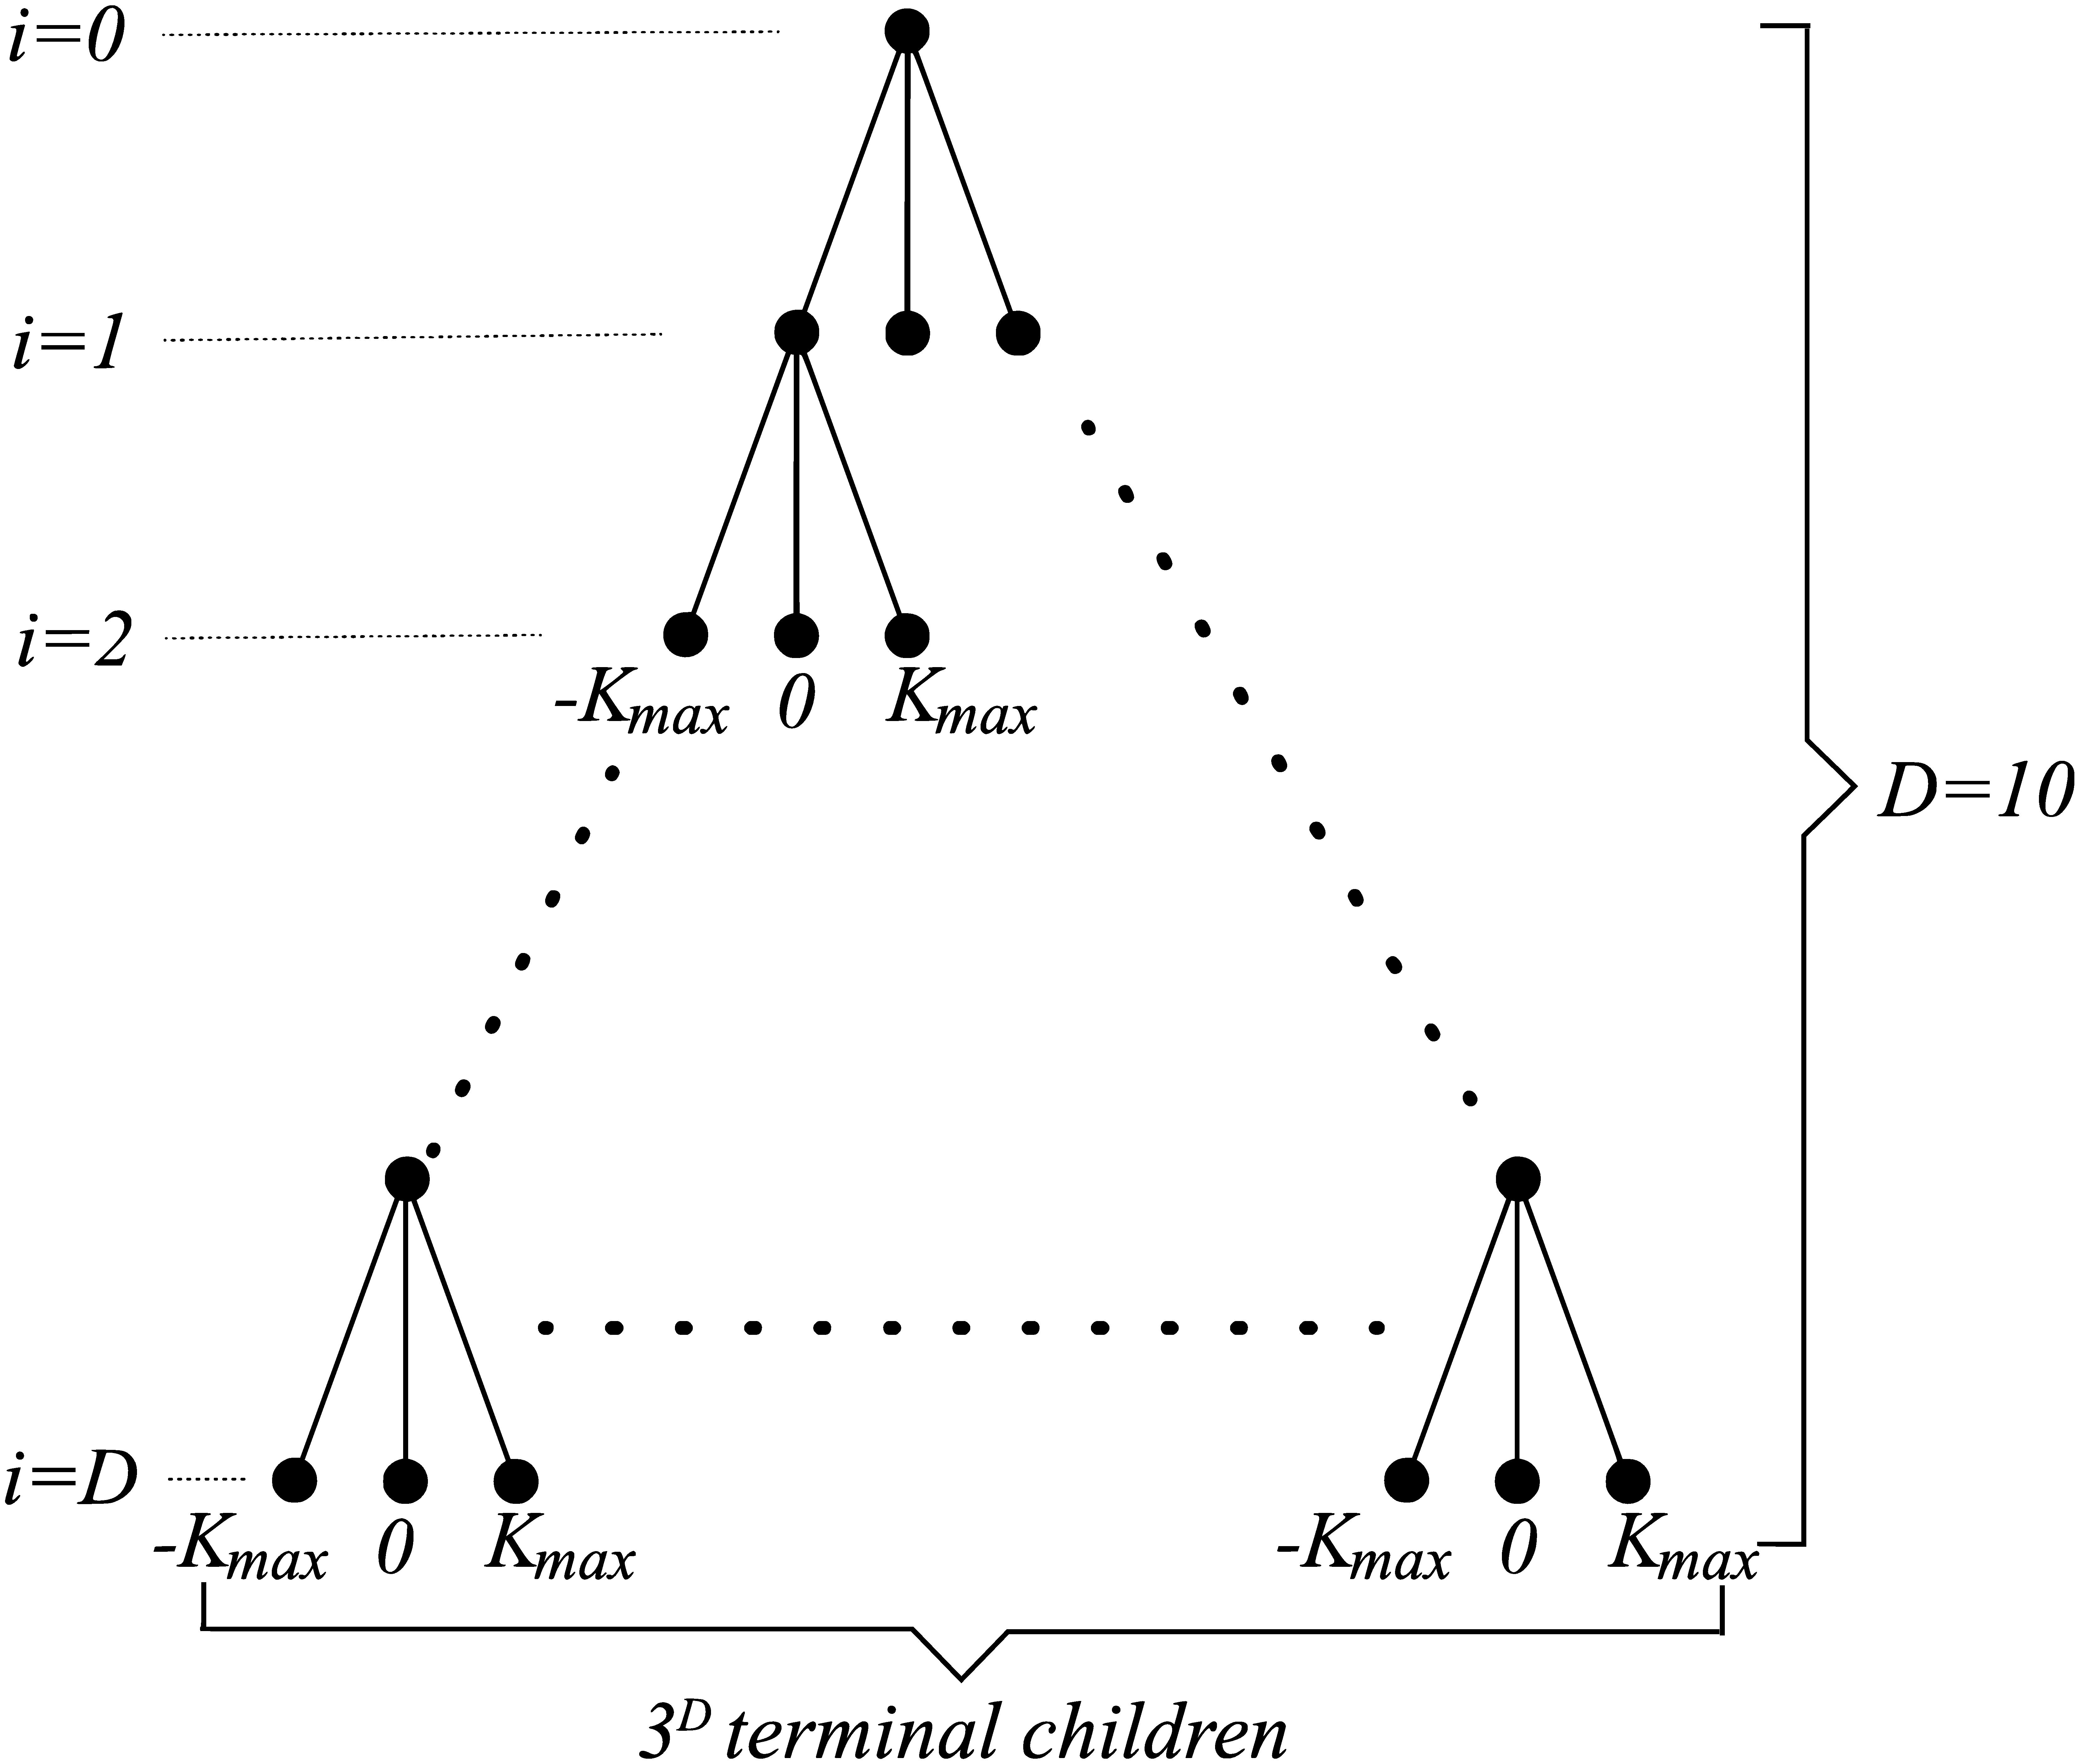
\includegraphics[width=5in]{tree2test.eps}
\caption{Tree structure}
\label{fig:tree2}
\end{figure}

To overcome the problem of the high computational cost needed to execute this amount of calculations, a variable search density approach is developed. This approach is implemented varying the number of children the algorithm skips to search, ${skip}_{rate}$, every time the value is worse than the best value. To prevent the search from skipping uncontrollably a large amount the children, a skip threshold, ${skip}_{th}$, is used. In Fig.(\ref{fig:skipexample}), a simple example for ${skip}_{th}=2$ is presented. Trying to maximize the cost function value, it is noticed that this technique manages to skip paths that lead to lower cost function value, saving computational resources and time. However, the solution is sub-optimal as the third child which results in the best cost function value has been skipped. The underlined numbers denote when the algorithm discovers a new best value and the $skip_{rate}$ is reset.

\begin{figure}[H]
\centering
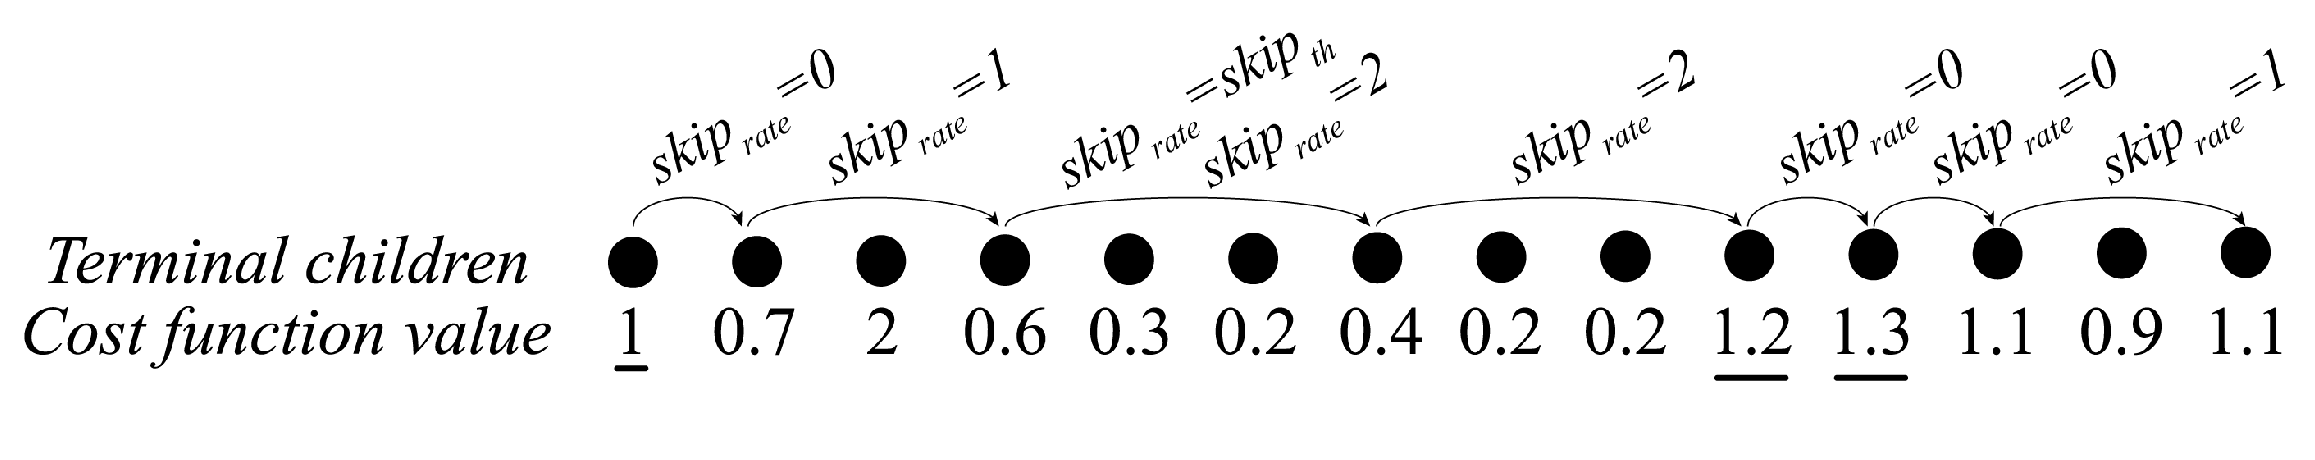
\includegraphics[width=1\textwidth]{skipexampletest.eps}
\caption{Skip child example}
\label{fig:skipexample}
\end{figure}

As a result, the branches of the tree become denser near high cost function values and sparser near lower values. Varying the "skip" parameter of the algorithm, a trade-off takes place between the computational time and how close to the optimal solution the result is. In Fig.(\ref{fig:tree.eps}), a visualization of the tree presents the dense and sparse areas where the lines are getting thicker and thinner respectively.
\begin{figure}[H]
\centering
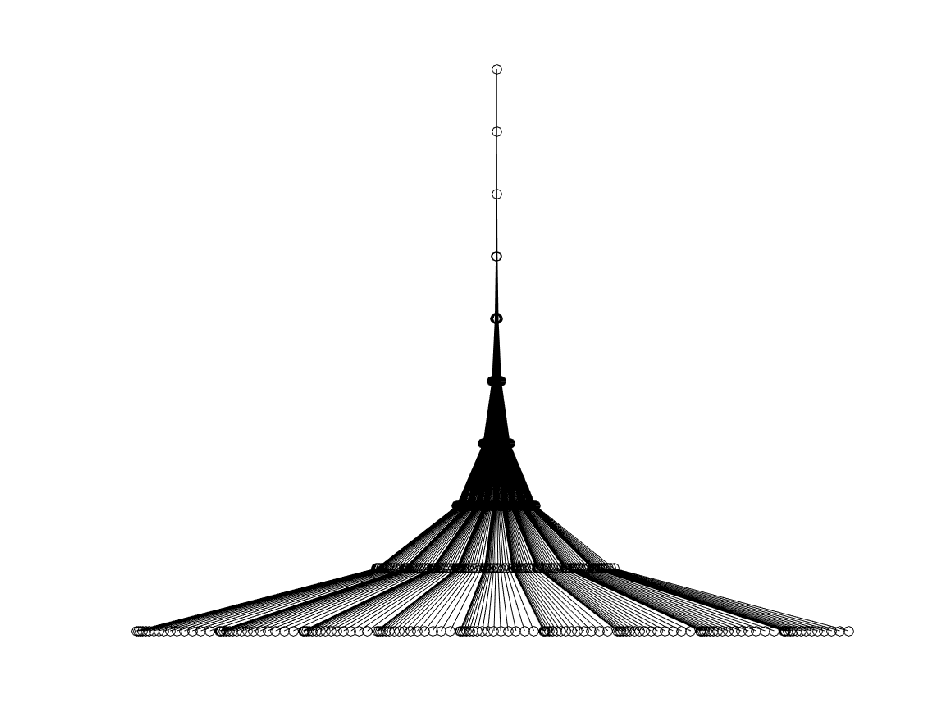
\includegraphics[width=0.6\textwidth]{tree.eps}
\caption{Tree visualization}
\label{fig:tree.eps}
\end{figure}


\section{Simulation Set-Up}
A specific task is selected to evaluate the efficiency of the method near an internal elliptic singularity. The 4-CMG cluster is in an elliptic singularity when the gimbal angles are equal to $\boldsymbol{\delta}=[-90, 0, 90, 0]^T $ deg \cite{bongwie2004}. This can be easily proven as follows:
\begin{equation}
\begin{matrix}
\textbf{A}(-90, 0, 90, 0)=\begin{bmatrix}
 0      &   0 &   0     &  0 \\
 1 &  -0.5774  &  1    & 0.5774 \\
 0 & 0.8164 & 0 & 0.8164\\
\end{bmatrix} \\ 
\textbf{N}=\mathrm{null}(\textbf{A})=
\begin{bmatrix}
 -0.7071 &  -0.3536 \\
 0.0000   & -0.6124 \\
 0.7071   & -0.3536\\
  -0.0000   & 0.6124\\
 \end{bmatrix} \\
 \textbf{u}=\mathrm{null}(\textbf{A}^T)=\begin{bmatrix}1, 0, 0\end{bmatrix}^T \\
 \textbf{E}=\mathrm{diag}(\textbf{u}^T\textbf{h}_N)=\mathrm{diag}(0.5774, -1, 0.5774, 1) \\
 \textbf{M}=\textbf{N}^T\textbf{E}\textbf{N}=
 \begin{bmatrix}
    0.5774  &  0 \\
    0  &  0.1444 \\
 \end{bmatrix}
\end{matrix}
\end{equation}
The determinant of matrix $\textbf{M}$ is obviously positive meaning that $\textbf{M}$ is definite and the configuration corresponds to an elliptic singularity. 
The exact simulation parameters used, are shown in Table.\ref{table:Parameters}.
\begin{table}[htbp]
\caption{\label{tab:Parameters} Simulation Parameters}
\centering
\centerline{
\begin{tabular}{lcccc}
\hline\hline
Parameter&Complex model& Kinematics only model\\\hline
Manoeuvre&0 to -90 deg& 0 to -90 deg\\
Moment of Inertia \textbf{J}& $\mathrm{diag}([1, 1, 1])$ $\mathrm{kgm^2}$& $\mathrm{diag}([1, 1, 1])$ $ \mathrm{kgm^2}$\\
Momentum $h_0$ & 1 Nms & 1 Nms  \\
Time-step dt&0.1 s&0.1 s\\
Simulation time& 7 s&7 s \\
PD, $K_p$, $K_\omega$ &20, 15& -----\\
$\textbf{h}_c$&-----&$\begin{bmatrix}1.5 & 0 & 0 \end{bmatrix}^T $ Nms\\
Skew angle $\beta$ & $54.73 $ deg&$ 54.73 $ deg\\
$\dot{{\delta}}_{th}$ &$ 50$ deg/s&$ 50$ deg/s\\
$\boldsymbol{\delta}_{ini}$ &$ [-70, 0, 75, 0]^T $ deg&$ [0, 0, 0, 0]^T $ deg\\
$k_{max}$ & 0.7& 0.7 \\
$\lambda_0$& 1 &1 \\
$\mu$ & 0.2 & 0.2\\
$w_{th}$&0.5&0.5\\
$g_1, g_2, g_3, g_4$&300,5,4,6&300,50,4,6\\
$D$&10&10\\
${skip}_{rate}$&variable in [0,250]&variable in [0,250] \\
${skip}_{th}$&250&250\\
\hline\hline
\end{tabular}
}
\label{table:Parameters}
\end{table}
The task is selected to be a manoeuvre in roll axis by -90 deg because the system encounters this elliptic singularity as long as the proper initial angles are used. Two different cases are examined. In the first, the kinematics and the dynamics equations of the system are implemented (complex model). The initial gimbal configuration is $\boldsymbol{\delta}_{ini}=[-70, 0, 75, 0] $ deg and the initial attitude quaternion is $\textbf{q}_{ini}=[1, 0, 0, 0]^T$. The system is commanded to follow the desired orientation given by the quaternion $\textbf{q}_{des}=[0.70711, -0.70711, 0, 0]^T$. A visualisation of the pyramid cluster in the initial configuration can be seen in Fig.(\ref{fig:cmgvisual.eps})
\begin{figure}[H]
\centering
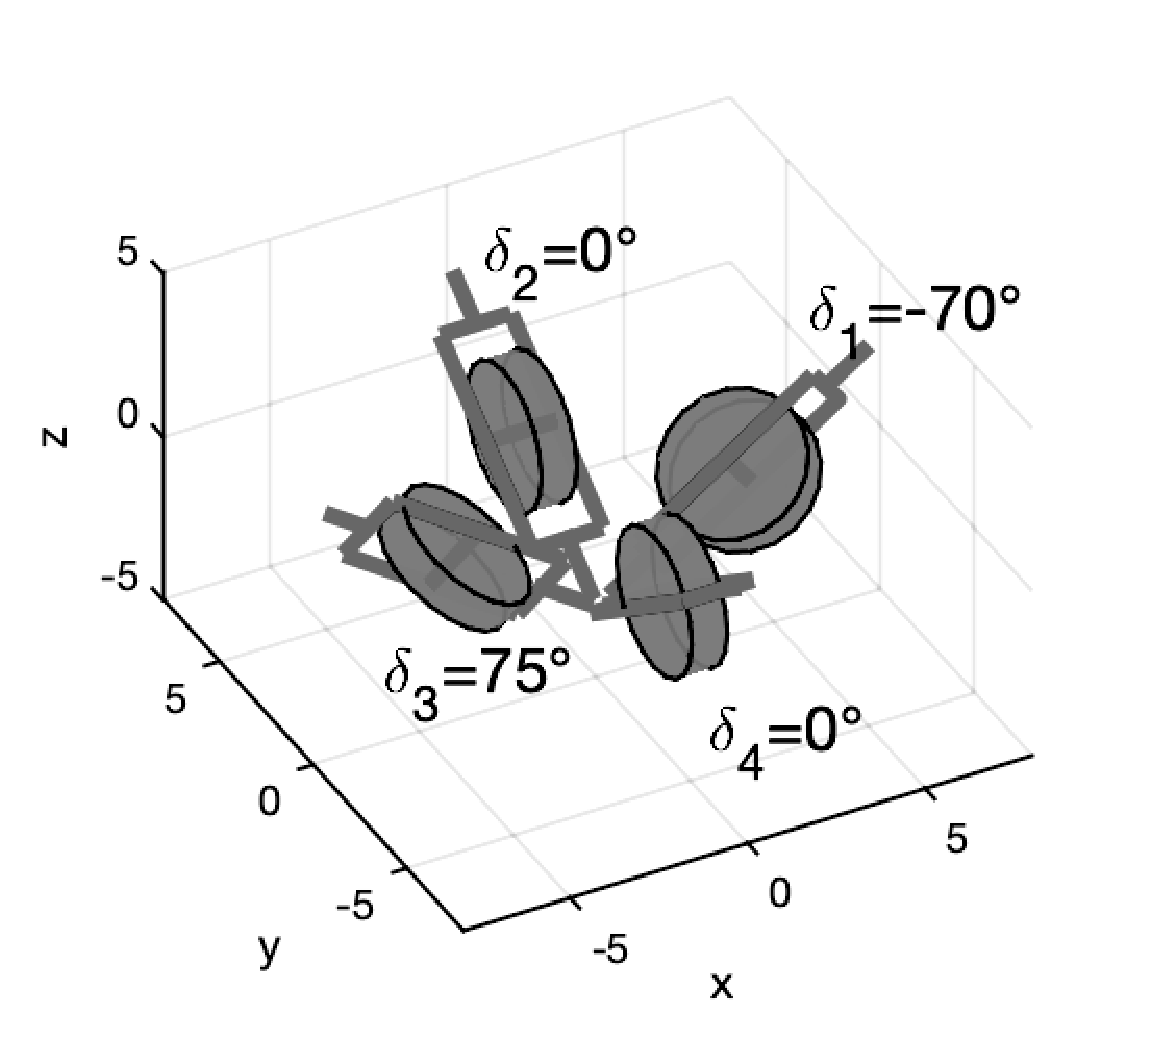
\includegraphics[width=3.5in]{cmgvisual.eps}
\caption{Cluster visualization}
\label{fig:cmgvisual.eps}
\end{figure}

Even if the initial configuration and the selected manoeuvre are not usual or practical for real-life satellite applications, dealing with the worst case scenario, is a simulation strategy which enables to prove that the proposed global steering method is effective in challenging conditions and showcases advantages and limitations as done in the literature\cite{lappasthesis,vadali_preferred,bongwie2005}. In this paper, a single axis manoeuvre is explored but the method is adaptable to every case as long as the initial configuration and the commanded manoeuvre are given. In the second case, only the kinematic model of the system is used, there is no PD controller and the input of the system is the difference between the current momentum and the commanded momentum over the time  $dt$. As no quaternions are used in this case, the third term in Eq.(\ref{eq:costfunction}) is replaced by the maximum norm torque error through the trajectory. The initial gimbal configuration is  $\boldsymbol{\delta}_{ini}=[0, 0, 0, 0] $ deg. For encountering an elliptic singularity for the specific initial configuration, the commanded momentum $\textbf{h}_c$ should be more than 1.15 Nms in \textit{x} axis \cite{bedrossian_momentum}, so $\textbf{h}_c=\begin{bmatrix}1.5 & 0 & 0 \end{bmatrix}^T $ Nms is selected. 
For the complex and the kinematics only model, the total simulation time is 7s. To better match the limitations of a real CMG cluster, the CMG gimbal angle rates reach the saturation when they exceed the specific threshold $\dot{{\delta}}_{th}$, through the following formula:
\begin{equation}
\label{eq:saturation}
\dot{\boldsymbol{\delta}}_{sat}=\dot{\boldsymbol{\delta}}\hspace{0.1cm}\frac{\dot{{\delta}}_{th}}{\max(|\dot{\delta}_1|,|\dot{\delta}_2|,|\dot{\delta}_3|,|\dot{\delta}_4|)}
\end{equation}
It is preferred to saturate the gimbal angle rates using Eq.(\ref{eq:saturation}) over applying a boundary value to every gimbal angle rate that exceeds the required threshold because the characteristics of the motion are conserved. 
To achieve null motion in each simulation time-step, $dt$, for a 15 s simulation, a tree depth $D=150$ is required. Such a depth is not practical for real applications and a much lower value is used ($D=10$). That means that the number of elements in $\textbf{L}$ set is different than $st$.  To obtain a $k_i$ value for every time-step, the $\textbf{L}$ set is interpolated through the simulation time. In Fig.(\ref{fig:interp}), two different approaches for interpolation are presented for a total simulation time equal to 0.15 s and $D=3$. $k_{max}$ is constant and is ignored in the figure for simplicity. The first (Fig.(\ref{fig:interp})a) approach is similar to a Zero-Order-Hold (ZOH) filter whilst the second(Fig.(\ref{fig:interp})b) is a linear interpolation.  In this paper, the linear interpolation is used.

\begin{figure}[H]
\centering
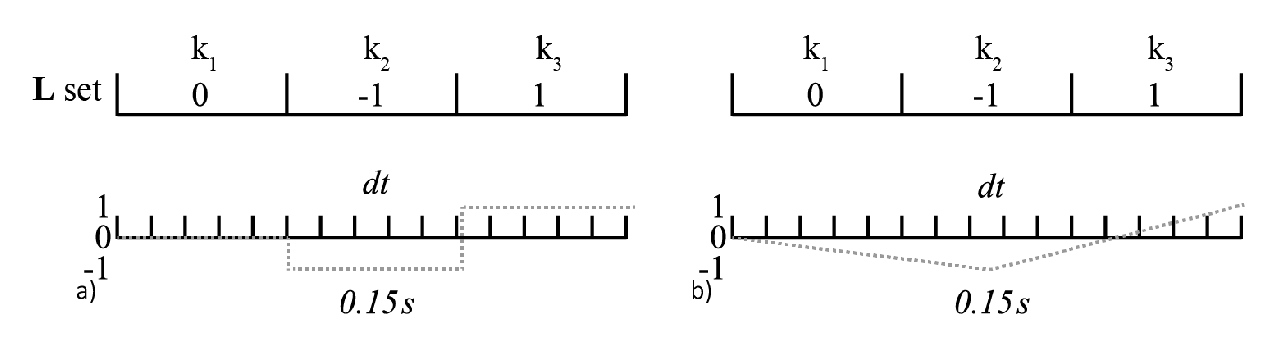
\includegraphics[width=1\textwidth]{interptest.eps}
\caption{Interpolation approaches. a)ZOH and b)Linear}
\label{fig:interp}
\end{figure}


\section{Simulation Results}
To evaluate the results derived by the method proposed in this paper, a comparison between a single axis CMG based manoeuvre which uses a conventional SRI steering logic and is compared to the method proposed in this paper.
\subsection{Complex model}
In the first simulation the search algorithm is not applied and the system makes use only of the SRI steering law as the singularity avoidance mechanism. The results are presented in Fig.(\ref{fig:without}). At t=0 s, the system is commanded to follow the desired attitude quaternion. The $\textbf{L}$ set in this case is $ \textbf{L}=k_{max}[0,0,0,0,0,0,0,0,0,0]$and the value of the cost function is equal to 0.129. As seen in Figs.(\ref{fig:without})a,d the attitude angle about the roll axis reaches the value of -86.25 deg at t=7 s.  The SRI steering law is responsible for the deviation in the attitude angle and the attitude error about the pitch and yaw axis from t=0.5 s to t=6 s as the system approaches the singularity. The maximum absolute deviation in pitch and yaw axis is 18 deg and 5 deg respectively. The maximum angular velocity as seen in Fig.(\ref{fig:without})b is about the roll axis but high velocities are presented to the rest axes as well. In the beginning, the angular momentum in \textit{x} axis is stuck to 1.15 Nms while the rest of the components are nearly zero (Fig.(\ref{fig:without})c) which is an indication that the system is in a singular state in this period of time as referred in the previous section. When the momentum in \textit{z} axis starts to rise, the satellite is starting to deviate from the desired trajectory and passes by the low performance configuration. The attitude error goes to zero at the end of the simulation, when the system passes the singularity reaching the commanded attitude. Fig.(\ref{fig:without})e shows that the gimbal angles in the beginning of the simulation are nearly $[-90,0,90,0]^T$until t=1.2 s indicating that the system is close to an elliptic singular state. As a result, no torque is generated by the cluster as shown in Fig.(\ref{fig:without})g for this time period. At the same time, the manipulability index (Fig.(\ref{fig:without})h) approaches and remains zero until the steering law starts to generate the off-axis error. Then, the system escapes the singularity and the value of the index in the steady state becomes equal to 0.609. In addition, the rate of the second gimbal remains saturated from t=2 s to t=3.3 s, scaling the rates of the rest gimbals according to Eq.(\ref{eq:saturation}).
Overall, the SRI steering law is capable of avoiding the low performance configurations generating attitude error but the specific tuning is driving the system fast into the singularity. It is expected that when the global optimization algorithm is applied, the null space motion re-configures the gimbal angles to values that is easier for the cluster to avoid the elliptic singularity.
\begin{figure}[H]
\centering
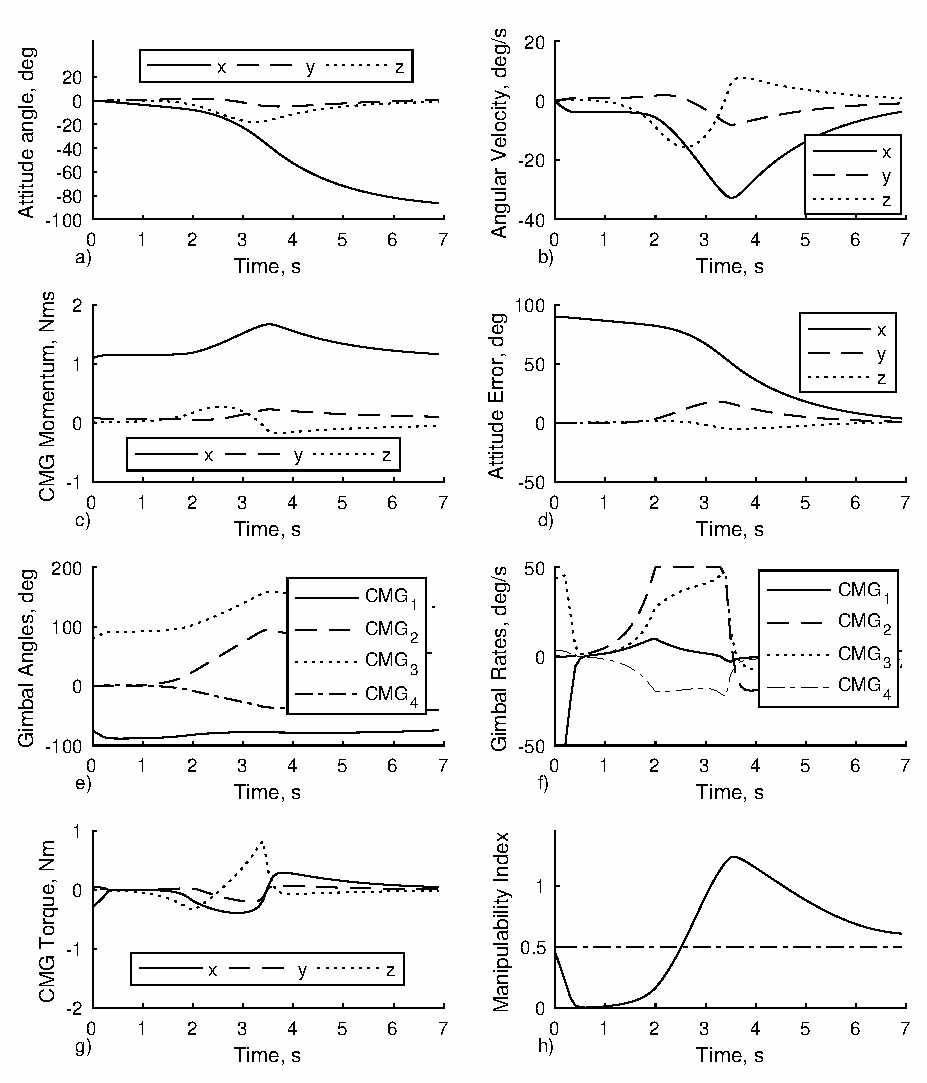
\includegraphics[width=6in]{0test.eps}
\caption{Results derived without using the search algorithm for dynamic and kinematic model. a) Attitude angle b)Angular velocity, c) CMG momentum, d) Attitude error, e) Gimbal angles, f) Gimbal rates, g) CMG torque, h) Manipulability index}
\label{fig:without}
\end{figure}
The second simulation utilizes the global optimization algorithm as described in Eqs.(\ref{eq:SR_inverse})-(\ref{eq:costfunction}) and the results are shown in Fig.(\ref{fig:with}). The $\textbf{L}$ set in this case is $ \textbf{L}=k_{max}[ 1,     1,     0,    -1,     0,     0,     0,     0, 0, 0]$ indicating the importance of the null space motion near the beginning of the motion slightly before the singularity occurs.
The manipulability index is taken into consideration near the beginning of the simulation in order to drive the system to a better performance configuration before SRI creates the off-axis error. 
This strategy assists the system to obtain a better mean manipulability value while SRI is creating the error upon the trajectory. 
In contrast, in the steady state no gimbal reconfiguration takes places. In Table.\ref{table:complexcomparison} the percentage change is presented for each $CF$ term compared to the first simulation.
\begin{table}[htbp]
\caption{\label{tab:complexcomparison} Complex Model - $\%$ Comparison}
\centering
\centerline{
\begin{tabular}{lc}
\hline\hline
$CF$ Term & $\%$ Change \\\hline
$w_{mean}$                        & 85.1 \%\\
$T_{w<w_{th}}$                       & -50 \%\\
$||\textbf{q}_{err}^v||_{max}$                &   7.5 \%\\
$T_{max\{\dot\delta_1, \dot\delta_2, \dot\delta_3, \dot\delta_4\}>\dot \delta_{th}}$& 47.1 \%\\
\hline\hline
\end{tabular}}
\label{table:complexcomparison}
\end{table}
There is an 99.3 \% increase in the cost function value compared to the first simulation and a significant improvement of 85.1 \% and 50 \% is presented in the mean value of the manipulability index and the $T_{w<w_{th}}$ term which is proportional to the time this index remains below the preset threshold. However, there is a slight difference in the attitude angle and error, the angular velocity and the CMG momentum profile as shown in Figs.(\ref{fig:with})a-d. The difference in the attitude angle and error profile is presented about the pitch and yaw axis that start to deviate from zero earlier. The same applies for the angular velocity of the satellite and the momentum of the CMG cluster. As shown in Fig.(\ref{fig:with})e, the second and the fourth gimbal angle starts to deviate from zero at t=0 s getting far from $[-90, 0, 90, 0]^T$ which is the key of preventing the system from spending a long time in the vicinity of the singularity. The combination of the null motion which starts in the beginning of the simulation and the simultaneous attitude error generated by the SRI results in a higher cost function value without significantly There is also a minor improvement in the settling time because the attitude angle about roll axis is -87.7 deg at t=7 s. The momentum of the cluster passes through $\begin{bmatrix}1.5 & 0 & 0 \end{bmatrix}^T $ Nms without being locked in this state but there is an noticeable increase in the time the gimbal motors remain saturated (Fig.(\ref{fig:with})f). 


This is the natural drawback to exploiting the null motion as the motors are used to rotate the gimbals to proper positions for a longer period of time. Even though a lower $k_{max}$ value reduces the time the gimbal rates spend in saturation, the cost function value becomes lower and the motion/results begin to look similar to those of the first simulation. 

A similar profile as in the first simulation is obtained for the CMG torque about the roll axis  (Fig.(\ref{fig:with})g), but no torque gaps are presented in between the motion as happens in the first simulation. The torque about roll spans in the negative of the axis until t=2.2 s when the direction changes in order to decelerate the satellite. A significant difference is observed in the manipulability index (Fig.(\ref{fig:with}h). It starts from the same value as in the first simulation but there is a noticeable decrease of 50 \% in the time it remains below the preset threshold and a 85.1 \% increase in its mean value. The horizontal dashed line indicates the value of the threshold $w_{th}$. 
Inevitably, the global optimization algorithm increases the power demands of the system as the gimbal motors are exploited not only for executing the desired manoeuvre but also for optimizing the given criteria. 

In general, the coefficients $g_1, g_2, g_3, g_4$  have to be selected according to the application. For example, a 20 times larger value of $g_4$ for the same $g_1, g_2, g_3$ values, results in different gimbal rates profile where the rates do not remain saturated for such a long period of time. However, the system remains near the singularity for a longer period of time. In this paper, the coefficients are selected mainly to improve the first and the second term. For real-life applications though, the power consumption and the motor gimbal stresses should be taken into consideration when tuning these parameters.
Hence, the selection of the weights constitutes a trade off between the terms that are desired to be optimized. It is expected that the performance of some of output variables deteriorate. It is difficult to satisfy all terms at the same time because they are contrary and this selection is application dependent. Moreover, the selected values of ${skip}_{rate}$ and ${skip}_{th}$ results in a sub-optimal solution for the optimization problem. Selecting lower values for ${skip}_{rate}$ and ${skip}_{th}$would produce a denser search with a solution closer to the optimal one.

\begin{figure}[H]
\centering
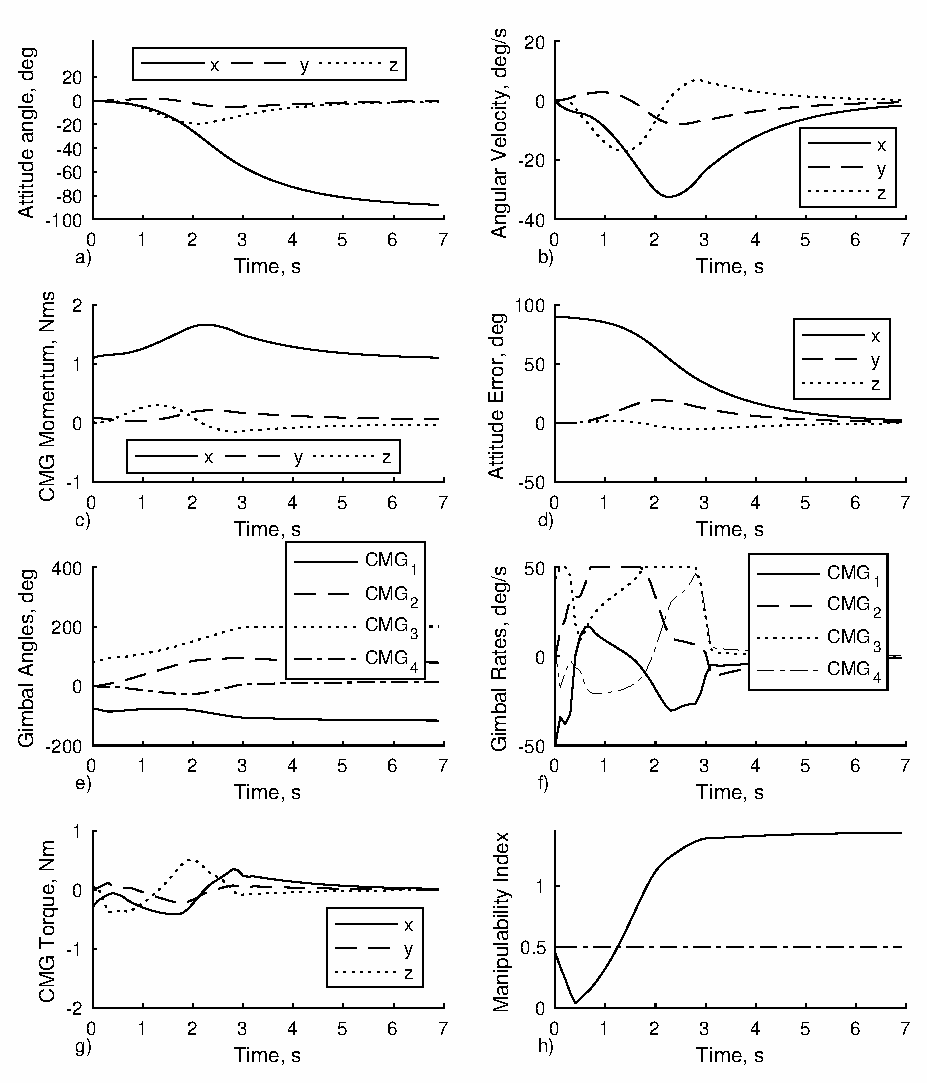
\includegraphics[width=6in]{1test.eps}
\caption{Results derived using the search algorithm for dynamic and kinematic (complex) model. a) Attitude angle b)Angular velocity, c) CMG momentum, d) Attitude error, e) Gimbal angles, f) Gimbal rates, g) CMG torque, h) Manipulability index}
\label{fig:with}
\end{figure}
For completeness, an additional arbitrary large angle 3-axis manoeuvre is selected to evaluate the efficiency of the proposed method. The commanded manoeuvre is given by the Euler angles $[62.7 ,  41.6,  -63.9]$ deg in "3-2-1" order. The results before and after the application of the global optimization algorithm are shown in Fig.(\ref{fig:3axiswithout}) and Fig.(\ref{fig:3axiswith}) respectively and Table.\ref{table:3axiscomparison} presents the \% changes for the CF terms. Even though the third term related to the attitude error remains almost the same as observed also in Fig.(\ref{fig:3axiswithout})a and Fig.(\ref{fig:3axiswith})a, there is a 103.4 \% improvement in the CF value. Fig.(\ref{fig:3axiswith})b shows that the gimbal rates remain saturated for a longer period of time compared to Fig.(\ref{fig:3axiswithout})b in order to re-orient the system to higher performance configuration. In Fig.(\ref{fig:3axiswith})c the null motion term as introduced in Eq.(\ref{eq:nullk}) is presented. It shows that both near the beginning and near the end of the simulation, the global optimization algorithm generates non zero gimbal rates in the null space. This is also demonstrated by the values of the $\textbf{L}=k_{max}[0  ,  -1,     1 ,    0  ,   0  ,   0 ,    0   ,  0  ,   1 ,   -1]$where the middle elements are mainly zero. As expected, the null motion term in the case where the global optimization algorithm is not applied is zero throughout the whole simulation time (Fig.(\ref{fig:3axiswithout})c) and as a result there is a 114.3 \% increase in the forth term which is proportional to the time the gimbal rates exceed the preset threshold. A significant improvement of 67 \% and 90.3 \% is presented in the mean value of the manipulability index and the time it remains below its threshold, respectively. It can be seen in Fig.(\ref{fig:3axiswith})d that the value of the index continues to increase after t=1.6 s resulting in higher performance configuration compared to Fig.(\ref{fig:3axiswithout})d where it dips and remains below the threshold from t=4.1 s to t=7 s.

\begin{figure}[H]
\centering
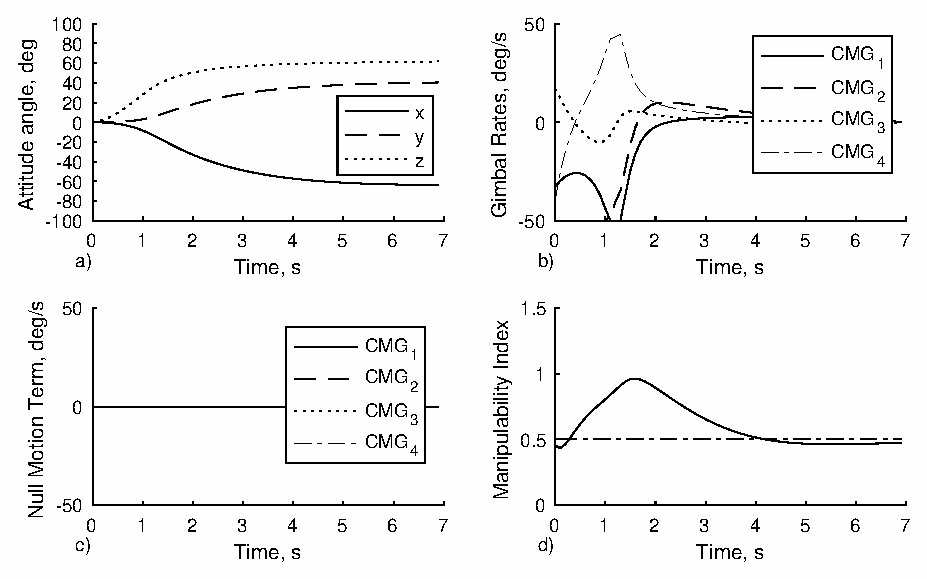
\includegraphics[width=6in]{3axiswithout.eps}
\caption{Results derived without using the search algorithm for a large angle 3-axis manoeuvre. a) Attitude angle b) Gimbal rates, c) Null motion term, d) Manipulability index}
\label{fig:3axiswithout}
\end{figure}

\begin{figure}[H]
\centering
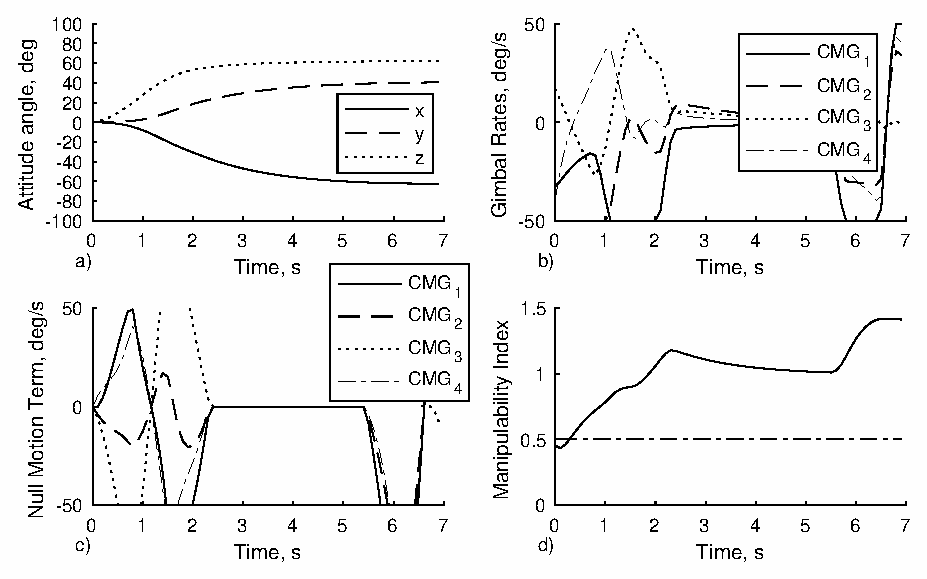
\includegraphics[width=6in]{3axiswith.eps}
\caption{Results derived using the search algorithm for a large angle 3-axis manoeuvre. a) Attitude angle b) Gimbal rates, c) Null motion term, d) Manipulability index}
\label{fig:3axiswith}
\end{figure}

\begin{table}[htbp]
\caption{\label{tab:3axiscomparison} 3-axis Manoeuvre - $\%$ Comparison}
\centering
\centerline{
\begin{tabular}{lc}
\hline\hline
$CF$ Term & $\%$ Change \\\hline
$w_{mean}$                        & 67 \%\\
$T_{w<w_{th}}$                       & -90.3 \%\\
$||\textbf{q}_{err}^v||_{max}$                &   $\approx$ 0 \%\\
$T_{max\{\dot\delta_1, \dot\delta_2, \dot\delta_3, \dot\delta_4\}>\dot \delta_{th}}$& 114.3 \%\\
\hline\hline
\end{tabular}}
\label{table:3axiscomparison}
\end{table}

\subsection{Kinematics}
In the third simulation no dynamics are used in the calculations for the manoeuvre. The results obtained when the search algorithm is not applied, are shown in Fig.(\ref{fig:kin0}). The $\textbf{L}$ set is the same as in the first simulation.
Fig.(\ref{fig:kin0})a shows that the steering law drives and "locks" the system in the singular state after the t=1.8 s. The configuration of the gimbal angles is $[-90,0,90,0]^T$ and no gimbal rates are generated by the steering law to drive the system away from this state (Fig.(\ref{fig:kin0})b). In addition, a non zero momentum error in \textit{x} direction is presented, as shown in Fig.(\ref{fig:kin0})c, which is equal to 0.35 Nms as the total CMG momentum becomes 1.15 Nms along \textit{x} axis. The manipulability index drops below the threshold at t=1.2 s approaching zero at t=1.8 s (Fig.(\ref{fig:kin0})d). The system remains locked in the singularity till the end of the simulation as the zero value of the index indicates.
\begin{figure}[H]
\centering
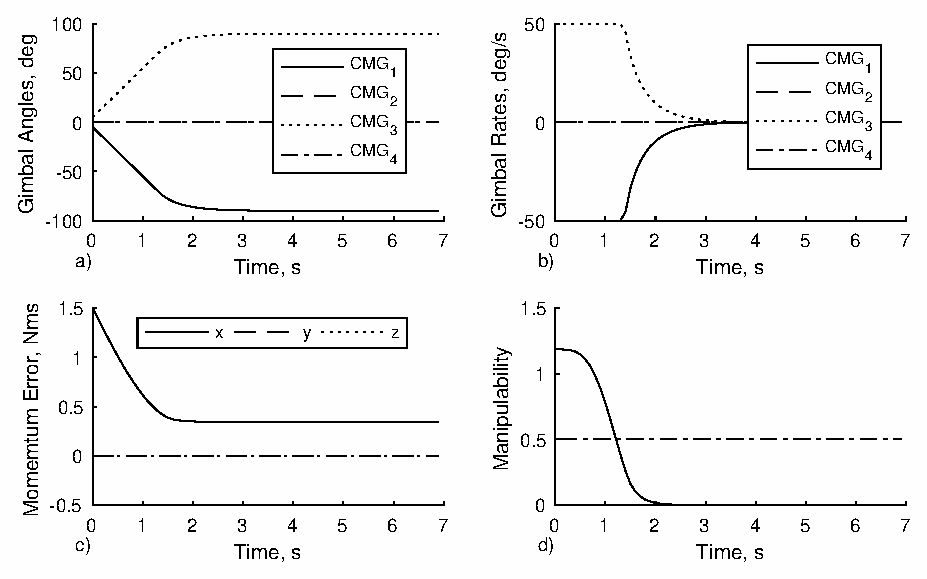
\includegraphics[width=6in]{kinwithouttest.eps}
\caption{Results derived without using the search algorithm for kinematic model. a) Gimbal angles, b) Gimbal rates, c) Momentum Error, d) Manipulability index}
\label{fig:kin0}
\end{figure}

In the fourth simulation, the global optimization algorithm is applied and $\textbf{L}=k_{max}[ -1  ,   1 ,    1 ,    1 ,    1,     0,    -1    , 0  ,   0,    -1 ]$. In Table.\ref{table:kinematicscomparison} the percentage change is presented for each $CF$ term compared to the third simulation and as in previous model a significant improvement in the first two terms is presented.
\begin{table}[htbp]
\caption{\label{tab:kinematicscomparison} Kinematics only Model - $\%$ Comparison}
\centering
\centerline{
\begin{tabular}{lc}
\hline\hline
$CF$ Term & $\%$ Change \\\hline
$w_{mean}$                        & 411 \%\\
$T_{w<w_{th}}$                       & -60 \%\\
$||\textbf{q}_{err}^v||_{max}$                &   0.64 \%\\
$T_{max\{\dot\delta_1, \dot\delta_2, \dot\delta_3, \dot\delta_4\}>\dot \delta_{th}}$& 235.7 \%\\
\hline\hline
\end{tabular}}
\label{table:kinematicscomparison}
\end{table}
As shown in (Fig.(\ref{fig:kin1})a,b) there is a noticeable difference in the gimbal angles and rates profile. The algorithm drives the gimbals to different configuration and there is a significant increase in the time the gimbal rates remain saturated. 
The momentum error converges to zero in every axis compared to the previous simulation but the SRI steering law generates error about the pitch and yaw axis as well (Fig(\ref{fig:kin1})c). In total, there is a negligible increase in the momentum error which is necessary to prevent the system from being locked in the singularity.
Significant difference is also noticed in the manipulability index as presented in Fig.(\ref{fig:kin1})d. At t=2.1 s the minimum value of the manipulability index is obtained which is high enough to consider that the system is not in singularity. The mean value as well as the time the index spends below the given threshold have both considerably improved. Moreover, after t=4 s that the system reaches the steady state, the optimization algorithm continues to improve the performance measure modifying the gimbal angles. Specific measures related to the attitude error and/or the manipulability index could be taken into consideration in applications where the power demands do not allow such an aggressive gimbal rates profile. For example, a modification to stop the optimization under a given attitude/momentum error threshold or above a preset manipulability value can be applied. In such cases, the assessment of the algorithm it is recommended to be done again. 
\begin{figure}[H]
\centering
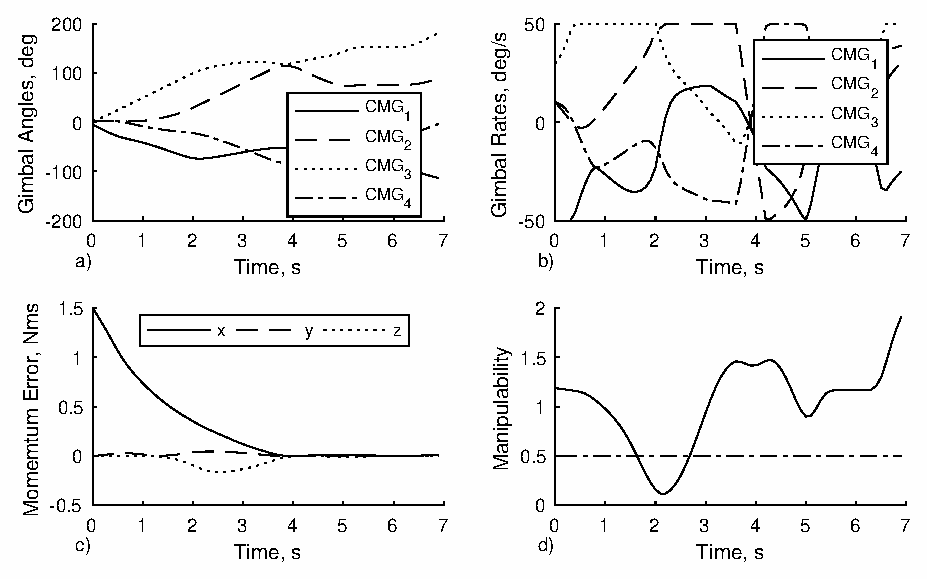
\includegraphics[width=6in]{kinwithtest.eps}
\caption{Results derived using the search algorithm for kinematic model. a) Gimbal angles, b) Gimbal rates, c) Momentum Error, d) Manipulability index}
\label{fig:kin1}
\end{figure}

For comparison, the k set before and after the interpolation is presented in Fig.(\ref{fig:kset})a and Fig.(\ref{fig:kset})b where $k_{max}=0.7$. 70 values are obtained, over the 10 initial values derived by the tree depth. 
\begin{figure}[H]
\centering
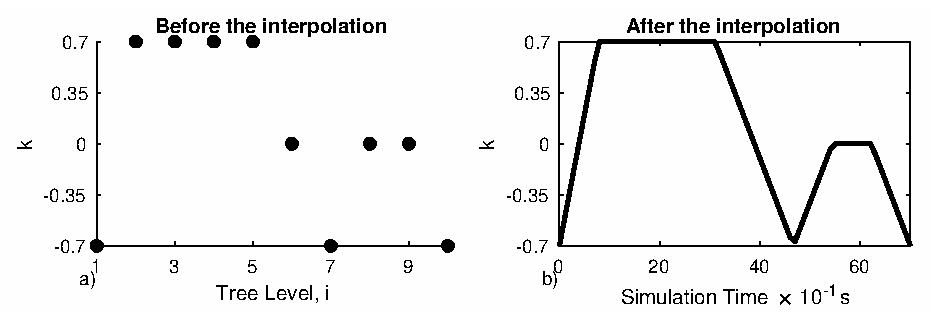
\includegraphics[width=6in]{ksettest2.eps}
\caption{\textbf{L} set a) before and b) after the interpolation}
\label{fig:kset}
\end{figure}
A linear interpolation is used for simplicity but any other interpolation method can be utilized. However, a cubic interpolation, for example, may change the result of the optimization algorithm deriving a different cost function value.

The computational efficiency of the algorithm is vital for real-life applications. The numerical results from the simulations are discussed below.
For the second simulation, there are 308 parent to child expansions whilst this number becomes equal to 284 for the fourth simulation. In the first case, the solution is found near the end of the search compared to the second case where the solution is found in the beginning of the optimization, skipping a number of nodes. The mean execution time for the complex and kinematics only model are also presented in Fig.(\ref{fig:timememory})a. 
\begin{figure}[H]
\centering
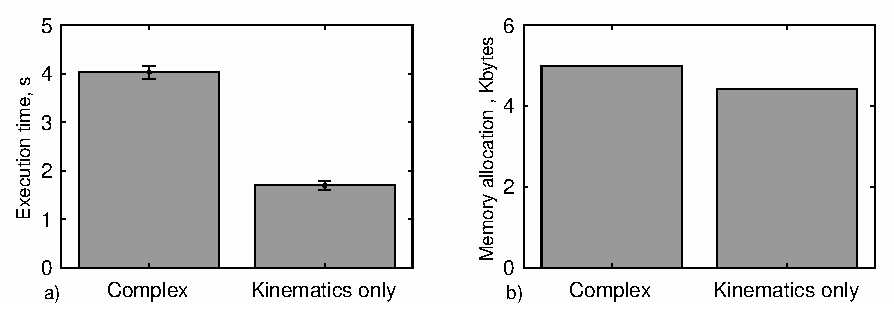
\includegraphics[width=6in]{timememorytest.eps}
\caption{Comparison among two models. a) Execution time and b) Memory allocation}
\label{fig:timememory}
\end{figure}
The mean execution time for the complex model is 4 s in contrast to the kinematics only model where the mean value is 1.7 s. This difference is expected not only because in the fourth simulation the solution is found near the beginning of the search but mainly due to the decreased numerical complexity of the kinematics only model. To better illustrate the computation difference the following index is calculated:
\begin{equation}
    \label{eq:i_exec}
    I_{exec}=\frac{ \textit{execution time in seconds}}{\textit{parent to child expansions}}
\end{equation}
For the complex model the index $I_{exec}$ has 2.2 times the value of the index for the kinematics only model, verifying that the complex model runs slower for the same parent to child expansions. In Fig.(\ref{fig:timememory})b are given, in numbers, the memory demands for each of these two simulations. 
It is observed that the code running the complex model allocates more memory as the code for the simple model. In applications with memory limitations, the kinematics only model can be exploited to predict the trajectory of the satellite. In combination with an inspection system it is feasible to monitor if the real system follows the prediction. In case of deviations present, e.g created by external disturbances, the kinematics model algorithm is executed again using as initial configuration the current configuration. This way, the kinematics only model can be used to handle a real system without dealing with the complex model and its shortcomings. However, in cases where higher memory allocation and execution time are allowed, the complex model is preferable because the in-between monitoring checks can be skipped.

In comparison with the approach used in \cite{paradiso},\cite{paradiso2}, our method clearly has an advantage over the execution time and the memory needs. There is an 60.7 \% improvement in the $I_{exec}$ and the comparison is held for the kinematics only model in order to be comparable to the model used in the literature. The storing precision in the previous study is limited to 1 byte per variable while in this paper the precision is 8 bytes per variable. This corresponds to approximately 950 Kbytes compared to 4.4 Kbytes used in this work. This is expected since there is not a node visit histogram to adjust the number of the children skipped. The proposed algorithm handles the complexity of the problem using the variable search density approach without requiring a large amount of memory. A histogram demands a significant amount of storing variables which is proportional to the total number of nodes. Moreover, the execution time as well as the computational resources needed by the algorithm can be adapted, adjusting only two variables, ${skip}_{rate}$ and ${skip}_{th}$. For example, decreasing the ${skip}_{th}$  increases the execution time and the parent to child expansions. On the other hand, a larger ${skip}_{th}$ value will better suit in applications where execution speed is vital. In this case, the result will be clearly sub-optimal.

The  $CF$ has been selected as a fraction whose numerator is desirable to be maximize and the denominator to be minimized. The only case for the denominator to be nearly zero is when all its terms are close to zero. This implies that the commanded manoeuvre is near the current attitude, the SRI does not create any deviation from the desired manoeuvre, the gimbal rates are below the saturation limit and the manipulability index is above the preset threshold through the whole simulation time. In this paper, the optimization algorithm is utilized to determine the null space motion for larger manoeuvres that pass near singular states where it is rare for all these terms to be zero at the same time. If this happens an exception handling mechanism is required to keep track of these states and prevent calculation errors. In such cases, it should be taken into consideration that it is possible to avoid a singular state due to the small computational residuals derived by the simulation environment, not by the actual control law, resulting in wrong conclusions. In this paper,  the point where the algorithm begins to consider a state singular is described by the manipulability threshold $w_{th}$ the value of which is selected to be 0.5, which is far enough from the ideal theoretical value of zero. Moreover, the singularity escape in Fig.(\ref{fig:without}) when the manipulability index goes to zero  is not related to numerical errors but it is a consequence of the large angle errors provided by the SRI application.


It is possible to use the same $CF$ to compare the same manoeuvre for different null space paths. However, altering the manoeuvre the results are not comparable mainly due to the third term of the $CF$ that includes the controller error and, in such cases, the third term can be ignored.
Additionally, the $CF$ could be simplified to optimizing the minimum value of the manipulability index across the trajectory as long as there is a singularity-free path for the desired manoeuvre. Otherwise, the maximum attitude deviation should be taken into consideration especially for real-life applications. The exploratory character of the current study does not demand the enforcement of such limitations in the attitude error. 
Near singularities, the actual gimbal trajectory is possible to deviate significantly from the propagated profile upon which the optimum null-motion profile was based. Thus, a code modification to adjust the size of $\textbf{L}$ set according to the manipulability index and thus the approach to singularity would significantly improve the reliability of the method. Furthermore, allowing more than three distinct values for the null space motion combined with a polynomial interpolation  would result in a smoother decision profile which is more appropriate for real applications.


\section{Conclusion}
In this paper, a global search optimization method is proposed. It makes use of the manipulability index, the time spend in the vicinity of singularity, the quaternion error and the gimbal rates to adjust the null motion upon the Singularity Robust Inverse (SRI) steering law. A ternary tree structure is used for the implementation and the results indicate that the proposed method is capable of reconfiguring efficiently the 4-control moment gyroscope (CMG) cluster with respect to a cost function that exploits information across the trajectory of an arbitrary desired manoeuvre in order to avoid an elliptic singular state. Such a singularity cannot be avoided through null motion after the system is locked in this state highlighting the importance of the global steering approach. Significant improvement is observed both in the kinematics only and the complex model regarding the manipulability related terms compared to the case where no null motion is added. The quaternion error presents a slight increase while the gimbal rates remain saturated for a longer period of time because the null motion is exploited. This effect can be reduced either changing the value of $k_{max}$ or the corresponding cost function coefficient. 

This work can be utilized either offline, for inspection of the motion before applying the commands to the satellite, or online demonstrating an easily adapted application to the situation needs. It does not use a node visit histogram, as utilized in previous applications to adjust the number of the children skipped resulting in lower computational cost. It provides a novel solution to optimizing long trajectories as the desired manoeuvre can easily be divided in an arbitrary number of steps while the computational resources required by the algorithm can easily be adjusted tuning only two variables.
To further this work a more tight coding of the search algorithm could considerably speed-up the execution time, enabling real-time operations with results closer to the optimal solution. Moreover, a modification to allow a variable $\textbf{L}$ set length with more than three distinct values is also reserved for future investigation.





\bibliography{bibliogr}

\end{document}
